Considera los dos triángulos que se muestran abajo en la Figura \ref{fig:20230323154049} (los triángulos no están dibujados a escala).

\begin{minipage}{0.6\textwidth}
    \textbf{¿Los dos triángulos son congruentes?}\\
    \emph{Escoge 1 respuesta:}\\
    \begin{choices}
        \choice Sí.
        \choice No.
        \CorrectChoice No hay suficiente información para decidir.
    \end{choices}
\end{minipage}%
\begin{minipage}{0.35\textwidth}
    \begin{figure}[H]
        \centering
        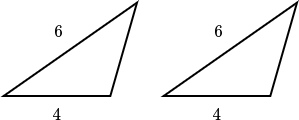
\includegraphics[width=\linewidth]{../images/20230323154049}
        \caption{}
        \label{fig:20230323154049}
    \end{figure}
\end{minipage}

\begin{solutionbox}{6cm}\footnotesize
    Dos triángulos son congruentes si tienen la misma forma y tamaño. En otras palabras, dos triángulos son congruentes si todos los lados y ángulos correspondientes son congruentes.

    \begin{minipage}{0.5\textwidth}
        Sin embargo, no necesitamos mostrar la congruencia de todos los lados y ángulos correspondientes para demostrar que dos triángulos son congruentes. Los criterios de congruencia (LLL, LAL, ALA) y el teorema AAL son atajos útiles para determinar congruencia de triángulos.
        En este caso, observa que dos lados de un triángulo son congruentes a dos lados del otro. Este no es un criterio de congruencia.
        Esto se debe a que es posible formar muchos triángulos con lados de longitud 44 y 66. La imagen de abajo muestra tres de esos triángulos.
    \end{minipage}%
    \begin{minipage}{0.45\textwidth}
        \begin{figure}[H]
            \centering
            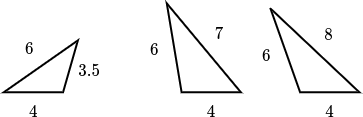
\includegraphics[width=0.9\textwidth]{../images/20230323154235}
            \caption{}
            \label{fig:20230323154235}
        \end{figure}
    \end{minipage}

    Los triángulos dados podrían ser congruentes si supiéramos que el ángulo entre los lados dados también es congruente, pero si no sabemos esto, no podemos sacar una conclusión.

    \textbf{No hay suficiente información para decir si los triángulos son congruentes o no.}
\end{solutionbox}